\section{国内外研究历史与现状}

% 3-4 页

由于众多路由异常事件对生产造成的巨大损失,已有一些技术和研究针对此问题进行了探讨\citing{sermpezis2018survey}。当前国内外对路由异常问题的研究主要分为缓解方法和检测方法两种大致方向:缓解方法通过在路由器引入一些针对性的协议从而阻止异常路由在网络之间转发;检测方法旨在通过一系列的算法和模型从实时更新的路由表中检测存在风险的路由。

\subsection{基于信任数据库的路由异常缓解方法}

资源公钥基础设施(RPKI)\citing{bush2013resource}是一个使用数字证书和公钥基础设施(PKI)来验证互联网路由信息的系统。它试图从源头和标准上控制路由异常的发生,旨在通过允许网络运营商对其路由公告进行加密签名并验证从其他网络收到的路由信息的真实性,以达到阻止 BGP 异常路由的产生。

RPKI 试图在分布式的广域网路由系统中建立中心化的信任数据库,并通过层次化的信任关系传递授权数据,反映到实际操作中即为运营商掌握的数字签名及其对应的私钥。如图 \ref{c1_rpki} 所示,RPKI 体系的工作方式与现代通用的证书系统大体上保持一致,运营商通过私钥签署自己信任的路由信息,并通过同样的方式吊销已签发的授权信息,这些信息将以数字证书的形式上传至 PKI 系统储存,并通过证书吊销列表(CRL)\citing{al2012development}的方式更新。 路由器在工作时,将连接至 PKI,通过证书的签名和有效性验证接收到的路由信息的真实性,进而选择接受或是丢弃路由。证书机制具有数学上可形式化验证的安全性,因而运营商可以确保接收到的路由是合法的,从而从源头上防止 BGP 劫持的发生\citing{wahlisch2012towards}。

\begin{figure}[h]
    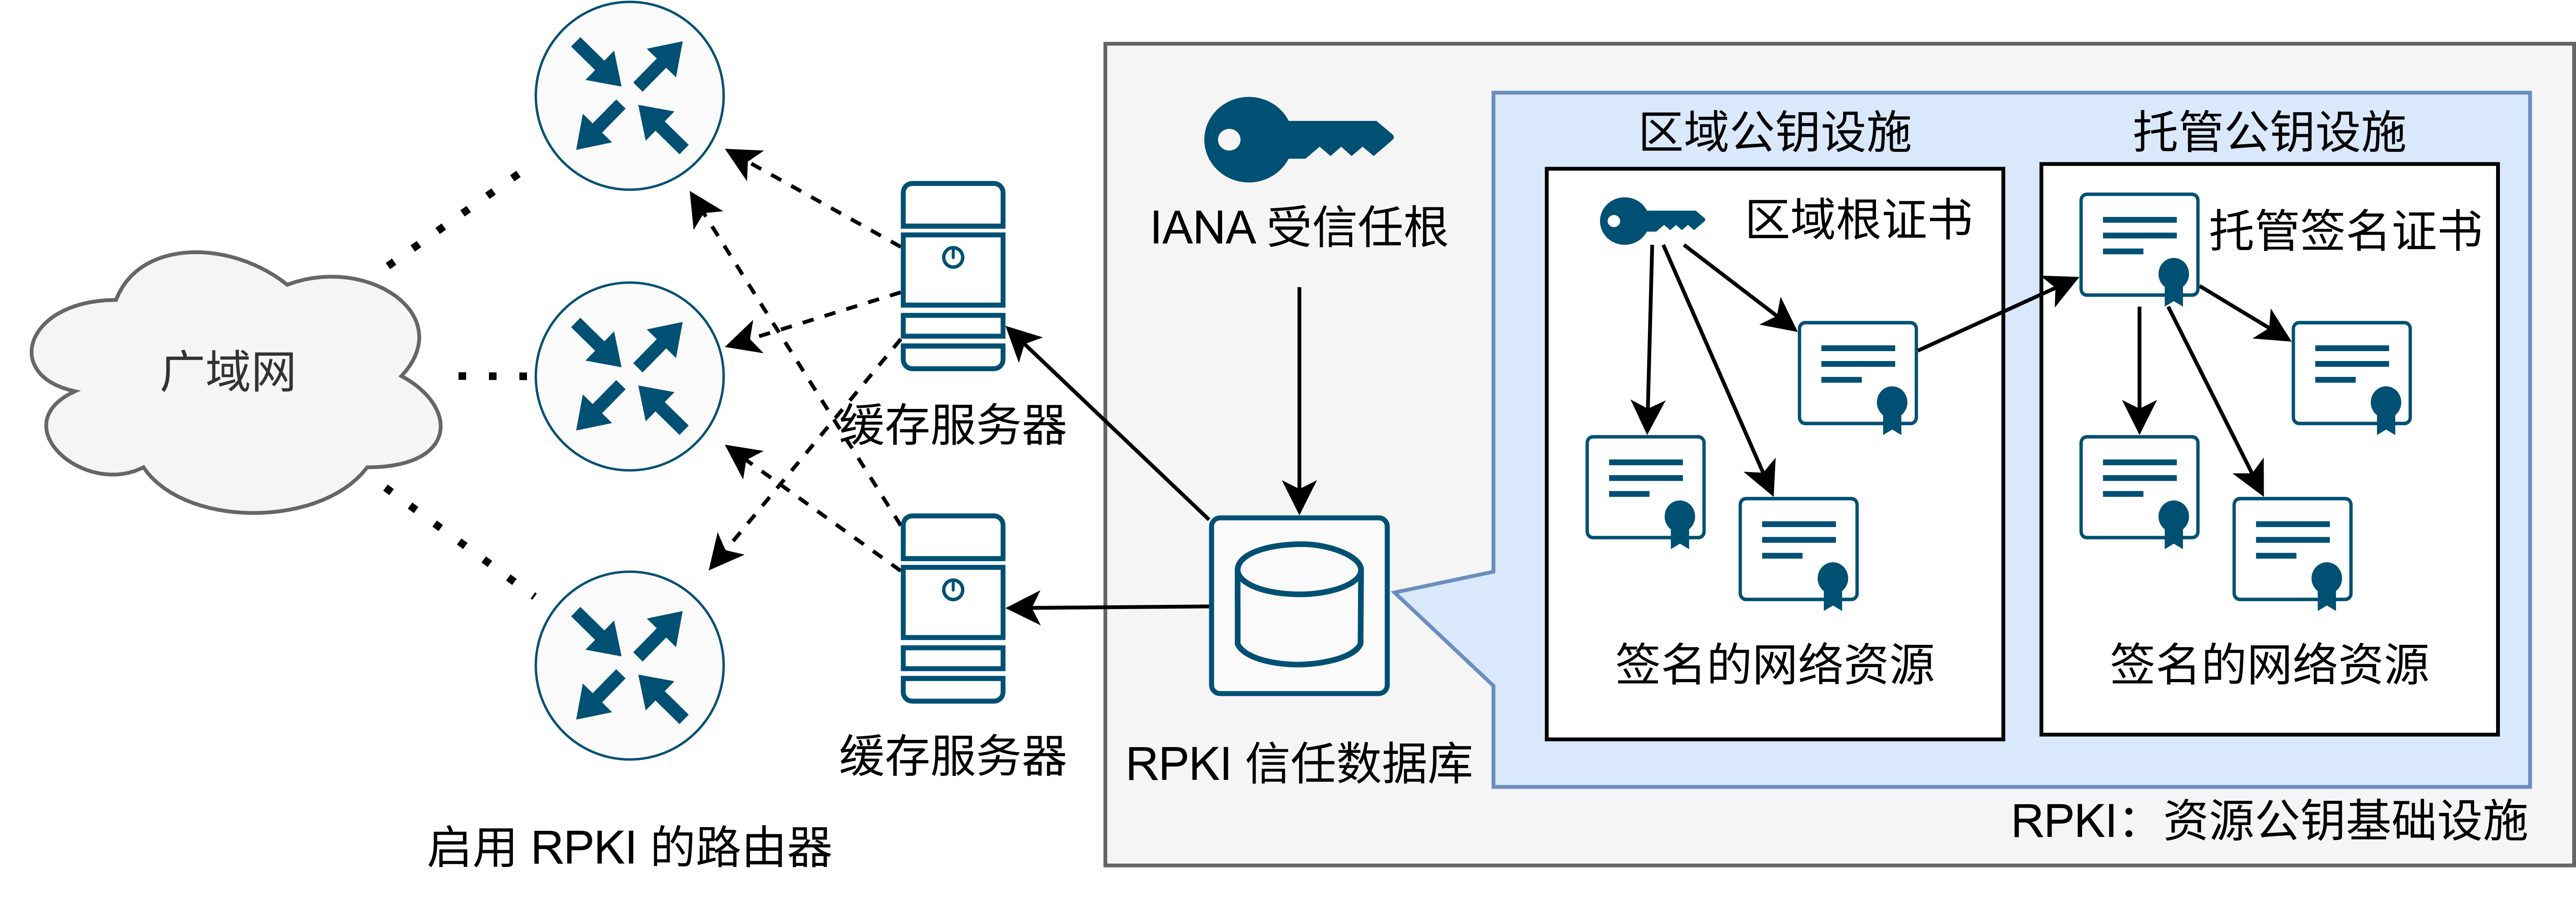
\includegraphics[width=0.9\linewidth]{chapter/c1_images/c1_rpki.png}
    \caption{RPKI 原理}
    \label{c1_rpki}
\end{figure}

然而它在 2013 年被提出至今,并未能有效避免广域网络中的路由异常,尤其是具有恶意目的的蓄意攻击;恰恰相反,无条件的信任机制反而引起了更多基于 PKI 机制的攻击。造成如此结果的原因主要有以下几点:

\begin{enumerate}
    \item 采用有限。RPKI是一个自愿的系统而不是一个强制性标准,并不是所有的互联网服务提供商(ISP)或自治系统(AS)都愿意在自己的网络中应用这一标准\citing{cooper2013risk}。这意味着仍有许多网络和设备没有使用 RPKI 来验证路由信息,这可能使它们容易受到BGP劫持。
    \item 复杂性。RPKI依靠使用数字证书和公钥基础设施(PKI)来验证路由信息。这引入了许多额外的流程,并且需要对 PKI 系统等安全设施进行适当的配置和维护\citing{cooper2013risk},否则会导致安全漏洞的产生。
    \item 人为错误。RPKI的信任模式决定了一些涉及密钥的操作必须人类完成,例如配置和维护 PKI 系统、配置路由验证策略等。\citing{cooper2013risk} 人为错误或失误可能导致系统出现错误,促使路由异常的产生。
    \item 恶意攻击。RPKI并非万无一失,可能会受到旨在绕过或破坏验证过程的恶意攻击。例如,攻击者可以通过入侵网络基础设施来获得有效的数字证书,并利用它来宣告非法的路由,或者对RPKI基础设施发起拒绝服务(DoS)攻击,以破坏验证过程\citing{wahlisch2015ripki}。
\end{enumerate}

因而,许多机构转而研究使用各类模型\citing{biersack2012visual} \citing{sermpezis2018artemis}对全球路由表进行建模,从而对路由异常进行早期预警和可视化分析。

\subsection{基于特征度量的路由异常检测方法}

% 0.8-1 页,包含优点缺点
% 缺陷:专家规则,单一或少量已知特征,很多时候基于已有数据和固定的建模方式。

一段时间内,基于统计特征的 BGP 异常检测被运用在多个运营商上,并取得了显著的成果\citing{al2016bgp}。它们主要分为两种类型:一类是通过时间序列特征寻找路由更新在时间上的关联性\citing{al2015detecting};另一类是从结构化的信息入手,从路径信息中提取包含异常的要素。 

一种朴素的异常检测思路是从类似决策树的 IF-ELSE 逻辑出发\citing{li2005internet},从路由的各项属性中发现异常路由发生时的统计量的变化,例如路由数量,更新数量,撤回数量等,这种方法在几场大型劫持事件中取得了较好的效果。 % li2005internet

根据同样的思路,一项研究通过特征工程的方式从 55 种 BGP 特征中提取出 9 种用于识别路由异常的关键特征\citing{hammood2021using},并指出它们相比其它特征而言在一些事件上更具代表性。 % hammood2021using

从时间序列数据入手是一种普遍的从时间特征出发的思路。例如从 BGP 条目更新的时间序列数据出发,使用自相似性\citing{prakash2009bgp}、指数和对数正态分布等统计学方法\citing{de2011anomaly}寻找重复出现的模式,这对于在时间上较为明显的路由异常而言是合适的思路。  % prakash2009bgp

而从结构化的特点入手则是另一种进行异常检测的方式。一种研究方法建立在路由目的地的所属地理信息上\citing{theodoridis2013novel},认为 AS Path 中出现的自治系统地区属性的频率和偏移与 BGP 可能的劫持相关联。 % theodoridis2013novel

而 AS Path 的高阶表示也能够反映出一定的异常特征。一项研究表明,通过发现监督学习中高阶路径的模式,能够对 BGP 事件进行有效的分类\citing{ganiz2006detection}。 % ganiz2006detection

以上方法大多声称自己具有较高的准确度,并已经在一些历史上存在精确记录的路由异常事件的数据集上得到了验证,然而,它们的缺点也比较显著:受限于现有的 BGP 异常历史数据、单一或少量已知特征和固定的拓扑模式,在面对更加复杂的网络环境时性能衰减非常显著。

\subsection{基于时序机器学习的路由异常检测方法}

% 0.8-1 页,包含优点缺点
% 缺陷:基于时间序列,不包含拓扑信息,存在误判可能,很多时候的路由劫持并不基于时间上的数量或单一指标特征。

由于传统基于特征度量的模型无法实现更新,为了能够在未知数据上获得更好的异常检测效果,一些以机器学习为基础的方法被提出。\citing{al2016bgp}它们主要从数据的时间序列特性上入手,通过相关统计量寻找潜在的异常时间点,其中长短期记忆单元(LSTM)与小波变换(Wavelet Transform)\citing{edwards2019border}是一类较为常见的方式。

利用 LSTM 神经网络对时间序列数据的敏感性,广域网路由表的更新能够被视为一个多维的流量时间序列\citing{cheng2016ms},并在时间的滑动窗口中从历史特征里学习潜在的模式\citing{al2012machine},在设置适当的时间尺度的情况下能够对路由异常做出精准的判断。  % cheng2016ms

小波分析在面对具有尺度缩放特点的时序数据上具有优势,因而通过 BGP 更新消息的时间方向自相似性能够借助小波变换对网络中的异常进行识别\citing{mai2008detecting},并通过聚类的方法缩小异常发生的范围。 % mai2008detecting

通过机器学习的时间序列方法构建的异常检测模型主要是将路由更新数据作为多维度的时序变量进行处理,因而在针对大规模路由异常数据上拥有较高的准确度。\citing{sriram2009comparative} \citing{theodoridis2013novel} 然而,这些方法同样存在特征不足的弊端,它们在将原始数据集转换为时间序列的同时,意味着丢弃了网络数据中的拓扑信息,此外,很多情况下,路由劫持并不一定影响全部的网络,事实上,大规模的路由异常往往是罕见的,利用基于时间上的数量或单一指标特征进行异常检测并不可靠。

\subsection{基于图网络的路由异常检测方法}

% 0.5 页,包含优点缺点
% 缺陷:本质上还是时间序列数据的特征变化,或没有考虑到路由算法本身基于路径的特点(BGP 的其它特征,例如 community)。

近年来,有研究开始尝试通过基于图的方式解决广域网的路由异常检测问题\citing{al2016bgp},将网络路由信息带入图的范畴。其中一种方式是利用相似度和相关性特点,将路由更新的相关指标间的依赖关系使用图网络来表示,此类做法事实上仍然基于时间序列数据特性的做法,存在与上述基于时序数据的模型一致的问题\citing{hoarau2022bgnn}; 另一种方式是使用在图上具有拓扑学习能力的 GNN 来解决异常检测问题,已有研究对此思路做出调研\citing{peng2022multi},实验证明使用基于图网络的机器学习方法来解决此类问题是具有研究前景的。% hoarau2022bgnn

将路由模型视作图网络是一种合乎逻辑的方式:广域网络的拓扑自身即是一类图网络\citing{sanchez2019comparing}。然而,模型没有考虑到基于路径本身的非拓扑属性(BGP 的其它特征,例如路由的社区属性),是当前使用图网络算法解决路由异常问题的一个常见的问题,同时由于路由数据的复杂性,仅采用传统的图神经网络的方式难以处理稠密且庞大的互联网路由数据。